\section{Latar Belakang}
\subsection{Sejarah Deep Learning}
Deep Learning mulai diperkenalkan di tahun 2006. Pada tahun 2006, Geoffrey Hinton (pada gambar \ref{labelgambar1} ) memperkenalkan salah satu varian jaringan saraf tiruan yang disebut deep belief nets, ide untuk men-train model jaringan saraf tiruan ini adalah dengan men-train dua layer kemudian tambahkan satu layer diatasnya, kemudian train hanya layer teratas dan begitu seterusnya. Dengan strategi ini dapat men-train model jaringan saraf tiruan dengan layer lebih banyak dari model-model sebelumnya.

\begin{figure}[h!]
	\centering
	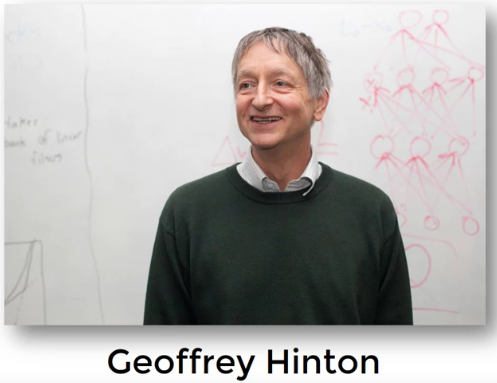
\includegraphics[scale=0.4]{figures/7.PNG}
	\caption{Gambar Geoffrey Hinton}
	\label{labelgambar1}
	\end{figure}

Setelah istilah deep learning populer, deep learning belum menjadi daya tarik yang besar bagi para peneliti karena jaringan saraf tiruan dengan banyak layer memiliki kompleksitas algoritma yang besar, sehingga membutuhkan komputer dengan spesifikasi tinggi, dan tidak efisien secara komputasi saat itu. Hingga pada tahun 2009 penggunaan GPU untuk deep learning diperkenalkan melalui paper yang berjudul Large-scale Deep Unsupervised Learning using Graphics Processors. Dengan menggunakan GPU jaringan saraf tiruan dapat berjalan lebih cepat dibanding dengan menggunakan CPU. Dengan tersedianya hardware yang memadai perkembangan deep learning mulai pesat, dan menghasilkan produk-produk yang dapat kita nikmati saat ini seperti pengenal wajah, self-driving car, pengenal suara, dan lain lain.


\subsection{Deep Learning}
Deep Learning (Pembelajaran Dalam) atau sering dikenal dengan istilah Pembelajaran Struktural Mendalam (Deep Structured Learning) atau Pembelajaran Hierarki (Hierarchical learning) adalah salah satu cabang dari ilmu pembelajaran mesin (Machine Learning) yang terdiri algoritma pemodelan abstraksi tingkat tinggi pada data menggunakan sekumpulan fungsi transformasi non-linear yang ditata berlapis-lapis dan mendalam.

Deep Learning adalah salah satu jenis algoritma jaringan saraf tiruan yang menggunakan metadata sebagai input dan mengolahnya menggunakan sejumlah lapisan tersembunyi (hidden layer) transformasi non linier dari data masukan untuk menghitung nilai output. Algortima pada Deep Learning memiliki fitur yang unik yaitu sebuah fitur yang mampu mengekstraksi secara otomatis. Hal ini berarti algoritma yang dimilikinya secara otomatis dapat menangkap fitur yang relevan sebagai keperluan dalam pemecahan suatu masalah. \cite{brownlee2014machine}

\subsection{Artificial Neural Network}
Neural network adalah model yang terinspirasi oleh bagaimana neuron dalam otak manusia bekerja. Tiap neuron pada otak manusia saling berhubungan dan informasi mengalir dari setiap neuron tersebut. Neural Network sebenarnya mengadopsi dari kemampuan otak manusia yang mampu memberikan stimulasi/rangsangan, melakukan proses, dan memberikan output. Output diperoleh dari variasi stimulasi dan proses yang terjadi di dalam otak manusia. Kemampuan manusia dalam memproses informasi merupakan hasil kompleksitas proses di dalam otak. Misalnya, yang terjadi pada anak-anak, mereka mampu belajar untuk melakukan pengenalan meskipun mereka tidak mengetahui algoritma apa yang digunakan.

Artificial Neural Network atau Jaringan Saraf Tiruan adalah sistem pemrosesan informasi yang memiliki karakteristik serupa dengan jaringan saraf biologis dan terdiri dari sejumlah besar elemen pemrosesan sederhana yang disebut neuron, unit, sel, atau node. \cite{irwansyah2015advanced}.

Teori dan permsalah yang akan dibahas dalam Deep Learning dapat dilihat dalam (tabel \ref{Permasalahan Deep Learning} )
\begin{table}[H]

\centering
\begin{tabular}{|c|c|c|}
\hline
No. & Teori & Tujuan\\
\hline
1   & Jaringan Saraf Buatan & Untuk memecahkan masalah pelanggan Churn\\
2   & Jaringan Saraf Konvosional & Untuk pengenalan wajah \\
3   & Jaringan Saraf Berulang & Untuk memprediksi harga saham\\
4   & Self-Organizing Maps & untuk menyelidiki Fraud\\
5   & Mesin Boltzmann & Untuk membuat sistem jaringan saraf berulang\\
\hline
\end{tabular}
\caption {Tabel Permasalahan yang dipelajari dalam Deep Learning}
\label{Permasalahan Deep Learning}
\end{table}




